\begin{figure}[H]
  \centering
  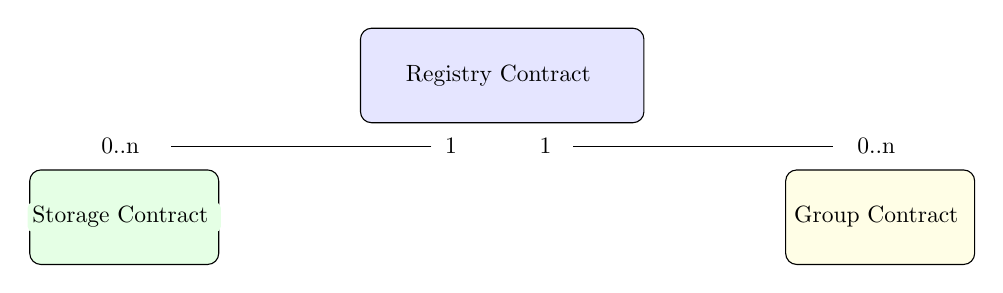
\begin{tikzpicture}[scale = 0.6, every node/.style={scale = 0.85}, every node/.append style={fill = white, rounded corners = 2pt, inner sep = 2pt, align = center}]

  \draw [rounded corners, fill=blue!10] (-3, 1) rectangle (3, -1);
  \node [fill=blue!10] at (0, 0) { Registry Contract };

  \draw [rounded corners, fill=green!10] (-10, -4) rectangle (-6, -2);
  \node [fill=green!10] at (-8, -3) { Storage Contract };

  \draw [rounded corners, fill=yellow!10] (6, -4) rectangle (10, -2);
  \node [fill=yellow!10] at (8, -3) { Group Contract };

  \draw (-1.5,  -1.5) -- (-7,  -1.5);
  \node at (-1, -1.5) { 1 };
  \node at (-8, -1.5) { 0..n };

  \draw (1.5,  -1.5) -- (7,  -1.5);
  \node at (1, -1.5) { 1 };
  \node at (8, -1.5) { 0..n };

  \end{tikzpicture} \\
  \caption{
  	Ethereum Micro-Architecture
  }{
    Outline of the micro-architecture of Ethereum contracts, shown with cardinality.
  }
  \label{fig:ethereum_micro_architecture}
\end{figure}
